\documentclass[1p,12pt]{elsarticle}

% Targets:
% Journal of Biomedical Informatics
% https://www.sciencedirect.com/journal/journal-of-biomedical-informatics
% Template Elsevier
%
% Computer methods and programs in biomedicine
% https://www.sciencedirect.com/journal/computer-methods-and-programs-in-biomedicine/publish/guide-for-authors
% Template Elsevier
%
% Journal of imaging informatics in medicine
% https://link.springer.com/journal/10278?srsltid=AfmBOoqkNdro6peThRxWn-1_kONFEDiY9bBHsKL5oLpz_fz5-N8aJ3Zu
% Template Springer

\usepackage[utf8]{inputenc}
\usepackage{graphicx}
\usepackage{hyperref}
\usepackage{booktabs}
\usepackage{multirow}
\usepackage{float}
\usepackage{caption}

% is having this necessary?
%\journal{Journal of Biomedical Informatics}

\makeatletter
\def\ps@pprintTitle{%
  \let\@oddhead\@empty
  \let\@evenhead\@empty
  \let\@oddfoot\@empty
  \let\@evenfoot\@empty
}
\makeatother

\begin{document}

\begin{frontmatter}

\title{MedGov-AI: An MCP-Based Agentic Framework for Clinical AI Integration and Medical Assistance}

% TODO: add author names, affiliations, and emails
\author[1]{Gabriel Santos}
\author[1]{Henrique Ferreira}
\author[2]{Martinho Tavares}
\author[2]{Luis Basti\~ao Silva}
\author[1]{José Luis Oliveira}
\address[1]{University of Aveiro, Aveiro, Portugal}
\address[2]{BMD Software, Ílhavo, Portugal}

\begin{abstract}
%Clinical AI integration and medical assistance remain fragmented: capable tools exist for imaging analysis, report generation, and clinical advising, but operate in isolation, requiring custom integration work that slows adoption. 
Clinical AI tools for medical imaging are increasingly capable but remain largely isolated from one another, requiring custom integration work that slows adoption and creates fragmented, difficult-to-maintain deployments. This paper presents MedGov-AI, an agentic system that addresses this through the Model Context Protocol (MCP) as a standardized interoperability layer. A large language model acts as an autonomous orchestrator, discovering and invoking clinical tools at runtime through MCP servers covering a broad range of tasks including DICOM parsing, CT segmentation, radiology report generation, whole-slide image cell segmentation, and digital pathology. Domain-specific workflow governance is provided through skill files that encode clinical sequences and guard conditions without model retraining. The system supports both interactive and event-driven operation, where files ingestion automatically trigger autonomous agent execution without user input.

Three end-to-end use cases were evaluated: CT analysis with structured radiology report generation; interactive whole-slide tumor detection with cell segmentation and pathology reporting; and autonomous workspace monitoring with cellular segmentation and file routing. We show that cloud-based LLMs completed multi-step clinical workflows reliably, within a bounded iteration cost, but locally-hosted 7--8B parameter models did not accomplish the same performance, revealing a tension between privacy and reliability in clinical deployment. The combination of skill-guided execution allows preventing clinically incorrect tool selection at ambiguous decision points. Summarily, six MCP servers were integrated in this open architecture without any agent-side connector code, supporting the argument that MCP can reduce the integration overhead currently limiting clinical AI adoption. The system's code and documentation are open-source at \url{https://github.com/BMDSoftware/MedGov-AI-MCP}, and a demo is publicly available at \url{https://medgovai.bmd-software.com/}.
\end{abstract}

\begin{keyword}
Agentic AI \sep Medical Imaging \sep MCP \sep MONAI \sep Clinical Workflow Automation
\end{keyword}

\end{frontmatter}

\section{Introduction}
\label{sec:introduction}

%Clinical AI integration and medical assistance are increasingly important topics, yet no implemented system covers the full scope: automated data analysis, structured report creation, clinical advising, and event-driven file analysis workflows. MCP has been evaluated as a protocol~\cite{mcp-aditi, mcphosts2025} and proposed as a conceptual integration layer for healthcare~\cite{transformingclinical2026}, but neither work applies it to clinical imaging workflows or provides an implemented, evaluated system. Medical imaging AI focuses on segmentation and detection accuracy rather than orchestration~\cite{agiformedicalimaging2025}, and agent skill systems have been formalized without application to clinical governance or comparison against a no-skill baseline~\cite{agentskillslargelanguage}. Each component exists in isolation; no prior work combines them into a working system and evaluates it end-to-end.

%MedGov-AI addresses this gap. It combines DICOM parsing, segmentation inference, and structured reporting under a single agentic orchestrator using MCP as the interoperability layer and skill files for workflow governance, evaluating both in end-to-end clinical workflows and providing empirical evidence for properties prior work argued only conceptually.

\subsection{AI in Clinical Practice}
Healthcare systems face rising imaging volumes against a constrained supply of specialists, creating diagnostic backlogs that affect patient outcomes. Automating routine analysis is therefore a structural necessity to improve consistency, to reduce clinician workload, and to free experts for complex cases. A wide range of AI tools is already available for clinical use, but with the notable characteristic that they typically operate in isolation, with no unified integration layer. In radiology, AI supports worklist prioritization and critical-finding alerts; in screening it acts as a first filter that lets programs scale~\cite{ruamviboonsuk2022retinopathy, wolf2024access}. Mayo Clinic has integrated AI into ECG and cardiac imaging as decision support~\cite{mayoclinic-ai-cardiology}, and in pathology whole-slide analysis is used for tumour grading and cell counting. For segmentation and detection specifically, FDA-cleared tools such as Viz.ai~\cite{vizai}, Aidoc~\cite{aidoc}, Transpara~\cite{transpara}, and IDx-DR~\cite{idxdr} are deployed across triage, screening, and grading.

These benefits carry significant risks. Bias arises when models trained on specific populations underperform elsewhere~\cite{mittermaier2023bias}, and can be introduced at any pipeline stage from dataset composition to deployment~\cite{kocak2025bias}. Hallucination is critical in report-generation models, where confident but incorrect statements carry direct patient risk~\cite{griot2025metacognition}, and the black-box nature of deep learning raises accountability concerns~\cite{kondylakis2026futureai}. No unified framework governs how clinical AI is validated, updated, or audited in production, and approval at development time does not cover hazards emerging after deployment~\cite{jia2025deployment}. Most relevant here, no established standards govern how agentic systems operate in clinical environments or log decisions for audit~\cite{trustworthyai2025}. The capability-to-deployment gap is substantial: fewer than 4\% of AI studies have been evaluated in real clinical settings~\cite{cozzolino2025surveillance}, with limited daily use reported among radiologists~\cite{kondylakis2026futureai, ce2024perceptions}.

Although the progress in individual tools, no standard layer orchestrates them within a workflow, forcing each institution to build and maintain its own connectors, which drives fragmentation, slow adoption, and costly maintenance. %The Model Context Protocol (MCP) is a promising solution, providing a standardized way for agents to discover and call tools without custom integration~\cite{mcp-aditi, mcphosts2025}, and has begun attracting clinical application~\cite{transformingclinical2026, kalathas2026mcp, ehtesham2025mcpfhir}. %This work extends that direction to multi-tool clinical imaging orchestration.

\subsection{Agentic AI in Healthcare}
Agentic AI refers to systems that autonomously set goals, plan multi-step actions, and use tools to achieve them~\cite{collaco2026scoping}. %Terminology is not standardized, some reserve the term for multi-agent orchestration, others apply it to any autonomous multi-step tool use~\cite{abouali2026survey}. We adopt the broader definition. 
Despite the risks of errors and biases, the advantages are enormous: systems do not fatigue, apply criteria uniformly, and process information faster than humans. Clinical imaging workflows, for instance, follow defined protocols with repetitive, predictable steps and well-defined outputs, making them strong candidates for autonomous orchestration.
However, the application of agentic AI in healthcare is still in a early phase, with only a few systems deployed and evaluated in real settings~\cite{collaco2026scoping, dietrich2025agentic}. 
Existing agentic frameworks, such as LangChain~\cite{langchain}, CrewAI~\cite{crewai}, and AutoGen~\cite{autogen}, lack to built custom agentic system because none natively a common tool protocol. Moreover, the integration of a custom loop also let us enforce clinical behaviours such as a completion contract (the agent cannot declare success while deliverables remain unmet) and an optional per-call confirmation mode. 
% We use a single-agent architecture, which offers greater simplicity, predictability, and accountability than multi-agent designs~\cite{collaco2026scoping} - properties that matter where every tool call must be traceable. Our system began as a hardcoded pipeline in which the LLM was never consulted and all sequencing was explicit conditional logic; this could not adapt without reprogramming, motivating the transition to a fully agentic design. The fundamental advantage is scalability: supporting a new domain requires only an MCP server exposing the relevant tools - community servers already exist for standards such as FHIR~\cite{ehtesham2025mcpfhir} - and the agent incorporates new servers at runtime without changes to the orchestration layer.

% We explored two backend approaches. The local option used Ollama's deepseek-r1:7b~\cite{deepseekr1} and llama3.1:8b~\cite{llama31}, small enough for consumer hardware and offering full data privacy. The local approach struggled with multi-step workflows: models frequently failed to select the correct tool and could not reliably chain calls, a limitation rooted in model scale rather than configuration. API-hosted models (Gemini 2.0/2.5 Flash, 3.0~\cite{gemini2025}) are also a more accessible path for institutions that cannot justify GPU infrastructure~\cite{agiformedicalimaging2025}, and resolved these issues immediately, at the cost of latency, third-party data transmission, and a dependence on external availability. Seamless, secure interoperability with existing platforms is a recurring prerequisite for agentic AI in care delivery~\cite{dietrich2025agentic}, a problem MCP directly addresses.

\subsection{MCP as a Standardized Tool Integration Layer}
The conventional approach to agent-tool integration has been based on REST adapters, written per tool to handle authentication, serialization, parsing, and error mapping. This solution does not scale, since each new tool adds an adapter, API changes break adapters, and the agent must encode assumptions about every tool. 
The Model Context Protocol (MCP) is a promising solution, providing a standardized way for agents to discover and call tools without custom integration~\cite{mcp-aditi}, and has begun attracting clinical application~\cite{kalathas2026mcp, ehtesham2025mcpfhir}. 
MCP defines a client-server protocol in which each server declares its tools at startup; the agent discovers and invokes them by name at runtime, decoupling it from individual tool APIs so that adding a server requires no agent changes. %Singh et al.\ survey MCP's architecture as the solution to fragmented integrations, and identify MCP sampling (LLM-to-LLM communication within the protocol) as a path toward sub-agent specialization~\cite{mcp-aditi}, noting healthcare's relevance but presenting no implemented system. 
A preliminary integration demonstrated 95\% correct tool selection from natural-language queries~\cite{mcphosts2025}, and MCP has been proposed conceptually as a foundational layer for clinical AI~\cite{transformingclinical2026}, but production-grade clinical deployments remain scarce.

\subsection{Skills as Clinical Capability Packages}
Tool access via MCP determines what an agent \emph{can} do, not what it \emph{should} do in a given domain, e.g, the correct sequencing of segmentation, terminology, and templating tools for a CT lung evaluation versus a pathology workflow is domain knowledge separate from both the agent's reasoning and the tools' logic. Skills can be used to address this layer. Xu and Yan formalize agent skills as composable, on-demand capability packages that guide an LLM without retraining~\cite{agentskillslargelanguage}, noting that skills and MCP are complementary: skills define what to do, MCP exposes the tools to do it. However, they do not address healthcare-specific  design, governance when protocols change, or composition with MCP in a working system.

\begin{table}[H]
  \caption*{\textbf{Statement of Significance}}
  \label{tab:significance}
  \centering
  \begin{tabular}{p{3.5cm}p{9cm}}
    \toprule
    \textbf{Problem or Issue} & Clinical AI tools operate in isolation with no standard integration layer, forcing institutions to build and maintain custom connectors that slow adoption and create fragmented, unmaintainable deployments. \\
    \midrule
    \textbf{What is Already Known} & Several AI tools for radiology and digital pathology do exist and are clinically deployed. However, orchatrating these services in a dynamic way is challenging and far to be achieved. By relying on a robust Agentic AI system, we can autonomously execute multi-step tool-calling tasks, by relying on MCP for agent-tool integration and on skills to guide LLM behavior without retraining. \\
    \midrule
    \textbf{What this Paper Adds} & An implemented agentic system integrating six clinical AI tools via MCP without custom connector code; empirical evidence that skills prevent domain mismatch at ambiguous decision forks; and a benchmark comparing API-hosted and local LLMs for clinical tool-calling reliability. \\
    \midrule
    \textbf{Who Benefits} & Physicians who can obtain pre-screenning results ahead of their analysis; researchers developing agentic AI for healthcare; software developers who aim to reduce integration overhead; institutions seeking auditable AI-assisted workflows.  \\
    \bottomrule
  \end{tabular}
\end{table}

\section{Methods}

\subsection{System Architecture Overview}

MedGov-AI is organized into three layers - a React frontend, a FastAPI orchestrator, and a set of MCP tool servers (Figure~\ref{fig:arch}) - with boundaries designed so that clinical domain logic lives entirely in the orchestrator, where it can be reasoned about, logged, and audited. The \textbf{frontend} is a React~18 application communicating with the orchestrator via a REST and a Server-Sent Events (SSE) API; SSE streams task progress and agent responses without polling.

\begin{figure}[H]
  \centering
  
\includegraphics[width=\textwidth]{images/AgenticArchitecture.pdf}
  \caption{MedGov-AI system architecture.}
  \label{fig:arch}
\end{figure}

The \textbf{orchestrator} is a FastAPI application that acts as the system's core. It is organized in three main services thar manage all the sessions, tasks' state, and MCP servers' connections. 
The \texttt{Agent} is the decision-maker running an iterative LLM loop, executing function calls across epochs, and maintaining session context so each result is available to the next.  We use a single agent rather than a hierarchy because multi-agent coordination introduces inter-agent communication and shared-state synchronisation~\cite{guo2024llmma}, an overhead that gives no gain to our solution. A single agent already achieves specialisation through MCP and keeps every tool call in one auditable session trace~\cite{collaco2026scoping}. 
The \texttt{Task Runner} manages long-running operations via a background thread pool tracked through a state machine. A semaphore limits concurrent GPU inference to one job, preventing out-of-memory crashes, and on failure passes captured \emph{stderr} to the LLM for a plain-language explanation. 
The \texttt{Watcher Service} polls registered directories and triggers the agent automatically when a file is deposited, enabling event-driven workflows from a PACS or scanner with no upstream changes. All state is persisted in a single SQLite database with write-ahead logging.

The orchestrator supports several LLM backends, selectable at deployment without changing agent logic. In the current implementation, we rely on the Gemini API for reliable multi-step function calling at the cost of external data transmission, and on Ollama for local inference with no external transmission. The tool layer consists of six MCP servers: five developed for this system and one community FHIR server for patient record retrieval. Each server runs as an independent process in its own virtual environment to prevent dependency conflicts %(most critically the GPU-enabled PyTorch required by \texttt{mcp-monai} versus the CPU-only install used elsewhere).
Tool names are auto-prefixed by server (e.g.\ \texttt{monai.run\_inference}), providing unambiguous namespacing. The five core servers are: \texttt{mcp-monai} (medical image segmentation and detection), \texttt{mcp-radlex} (RadLex terminology and report templates), \texttt{mcp-utils} (DICOM parsing, filesystem operations, and skill file access), \texttt{mcp-ipath} (telepathology integration), and \texttt{mcp-cellpose} (2D/3D cell segmentation).

The FHIR-based patient record integration was performed by connecting an existing community FHIR MCP server~\cite{ehtesham2025mcpfhir}, demonstrating that third-party servers can be plug into the architecture without changes in the orchestration layer. Extending the system thus requires only registering a compatible MCP server in the configuration file; the agent, orchestrator, and existing servers remain unchanged. This is the property that makes MCP a viable interoperability layer rather than a bespoke integration approach.

\subsection{MCP Server Layer}
Each server encapsulates a distinct capability as named, schema-defined tools that the agent discovers at startup and selects among by context. 
\textbf{Mcp-monai} is the inference server, built on MONAI~\cite{monai} with PyTorch. It detects modality and body part from DICOM metadata (with pixel statistics as a fallback heuristic), returns a ranked list of compatible models retrieved from HuggingFace Hub on demand, and runs inference with a sliding-window strategy that applies the model to overlapping sub-volumes to avoid GPU memory overflow on large 3D scans. Bundled models cover spleen, pancreas/tumour, lung-nodule, and whole-body (104 structures) CT segmentation, brain-tumour MRI, and UNEsT kidney segmentation. 
\textbf{Mcp-radlex} provides structured radiology reporting via the RadLex terminology standard; when populating a report it uses MCP sampling to delegate the mapping of segmentation outputs to template fields back to the host LLM, which also generates the findings narrative, closing the loop between inference and standardized documentation. 
\textbf{Mcp-utils} provides DICOM metadata extraction (per file or directory), general filesystem operations (read, write, move, copy, delete, list, search), and skill file access via \texttt{read\_file}, allowing the agent to load skill bodies on demand from the filesystem.
\textbf{Mcp-cellpose} provides cell segmentation using the Cellpose v4 universal model (cpsam)~\cite{cellpose}; v4 replaced v3's task-specific models (cyto3/cyto2/nuclei, $\approx$80~MB each) with a single SAM-based model ($\approx$2.5~GB), producing better results and more complete boundaries in densely packed regions (Figure~\ref{fig:cellpose-comparison}). The current implementation uses grayscale mode and detects GPU at startup with CPU fallback, practical only for small images.
\textbf{Mcp-ipath} integrates the iPath telepathology platform~\cite{Jesus2023}, aggregating whole-slide images (WSI) and DICOM via Dicoogle and DICOMweb, supporting thumbnail retrieval, resolution-level coordinate mapping, and region-of-interest extraction without downloading the full WSI.

\begin{figure}[H]
  \centering
  \begin{tabular}{ccc}
    
\includegraphics[width=0.30\textwidth]{images/cellpose_cyto_mask.jpeg} &
    
\includegraphics[width=0.30\textwidth]{images/cellpose_cpsam_mask.png} &
    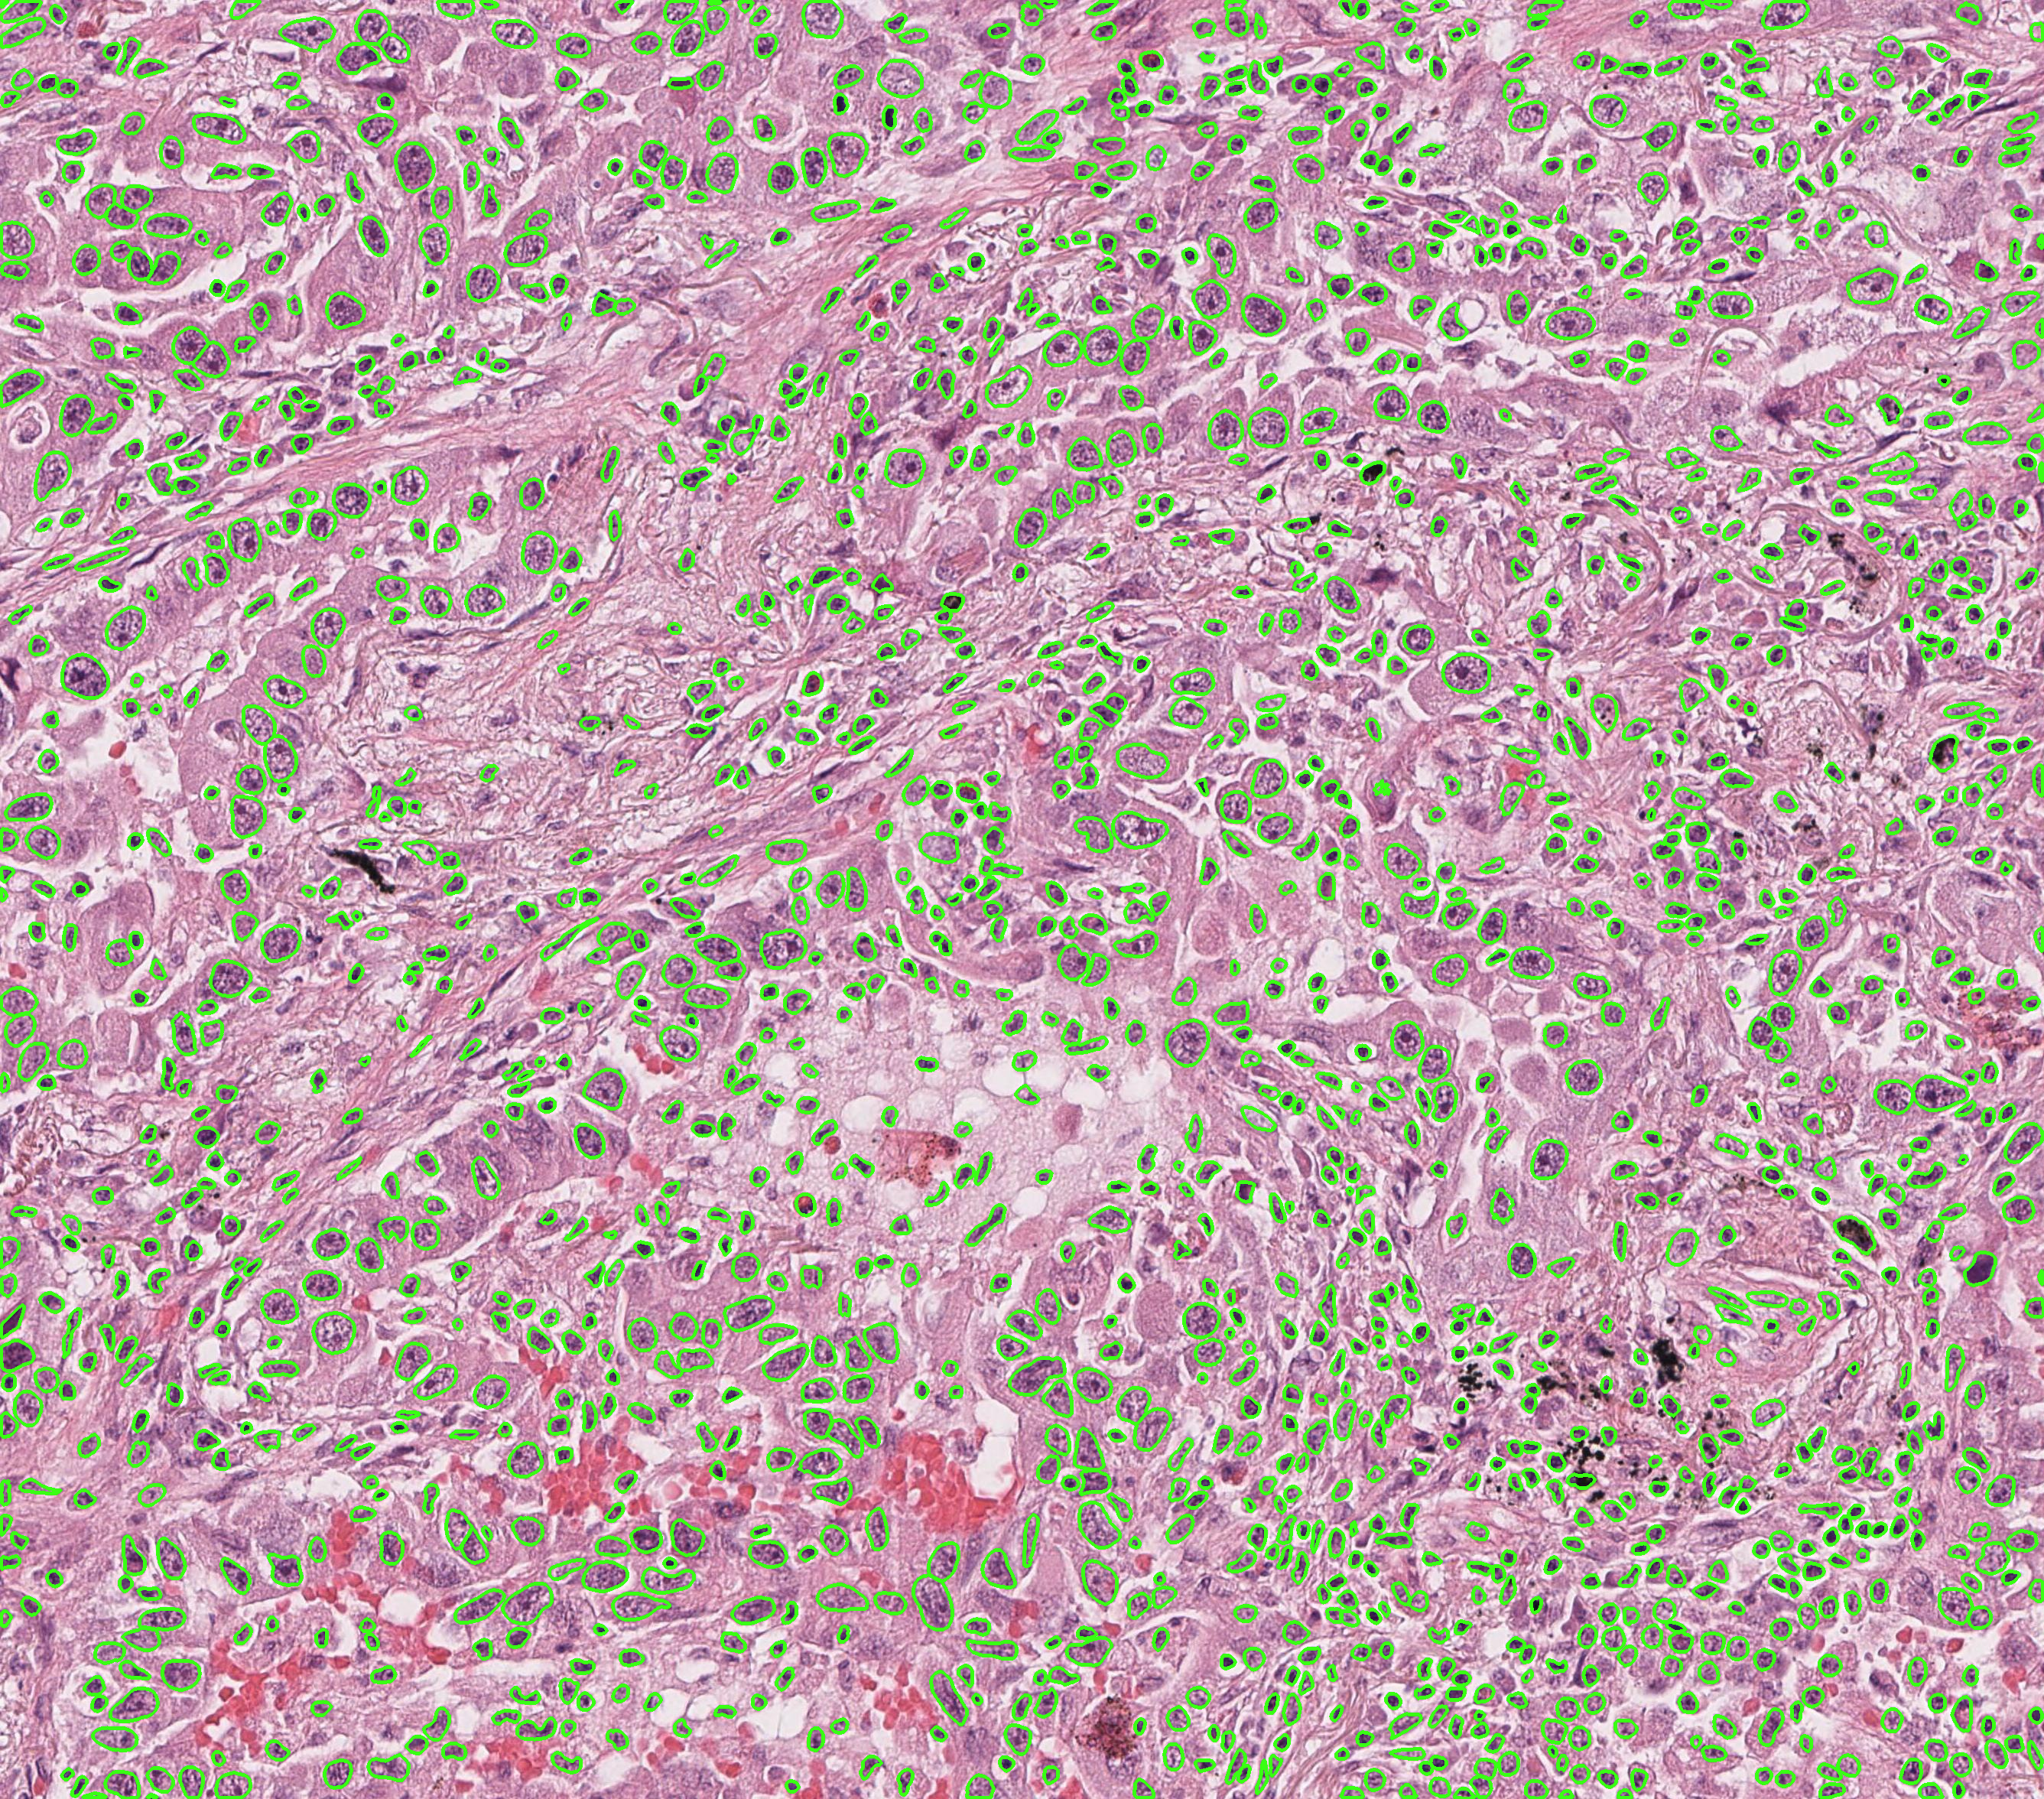
\includegraphics[width=0.30\textwidth]{images/cellpose_cpsam_overlay.png} \\
    \small v3 cyto (1{,}123 cells) &
    \small v4 cpsam (1{,}706 cells) &
    \small v4 cpsam overlay on H\&E \\
  \end{tabular}
  \caption{Cellpose version comparison on the same pathology ROI. Binary segmentation masks from v3 (cyto) and v4 (cpsam) are shown alongside the v4 mask overlaid on the original H\&E (Hematoxylin and Eosin) image. The v4 produces denser and more complete cell detection in packed regions.}
  \label{fig:cellpose-comparison}
\end{figure}

\subsection{Skills System}
\label{sec:skills}
The skills system encodes domain-specific guidance that the agent loads on demand. A skill body can be a step-by-step workflow protocol with sequencing constraints and cross-server coordination, or a body of domain knowledge such as regulatory standards or report templates. This guidance cannot be derived from tool schemas alone and is too domain-specific or voluminous to embed permanently in the system prompt. Embedding it permanently would increase token consumption on every request and raise the risk of instructions being overlooked in a large prompt.

A skill separates \emph{awareness} from \emph{detail}: every skill is surfaced at startup through a short name and description kept in the system prompt, while the full body stays unloaded until needed. When a request arrives, the agent reasons over these descriptions, identifies the applicable skill, and loads its body as operating instructions from the filesystem, enabling progressive disclosure, a lightweight index at rest, expanding to full detail only for the domain in use. A skill body can itself be hierarchical, routing from an entry document to sub-documents, references, templates, and scripts loaded independently as needed. Four skills are deployed: \textbf{dicom-analysis} encodes the tool sequence and guard conditions for DICOM analysis ending in a radiology report; \textbf{wsi-tumor-detection} encodes the inspection and cell-counting workflow for WSI pathology; and the community skills \textbf{clinical-reports} (regulatory standards and structured documentation templates) and \textbf{pydicom} (API guidance for DICOM manipulation) illustrate skills as knowledge packages adoptable without modification. A key governance property is that skill files are plain text and can be updated without touching the agent, servers, or codebase: editing the relevant reference document changes behaviour on the next session with no software deployment, separating workflow maintenance from software development - relevant where the people who understand a procedure are not those who maintain the code.

\subsection{Agentic Execution Loop}
The agent is governed by an iterative loop that drives the system from a natural-language goal to completed deliverables, calling MCP tools based on the LLM's reasoning at each step. At session start the agent receives a system prompt establishing its role, tools, and rules, including the available skills (name and description) injected after dynamic discovery, and explicit guidance on when to read a skill before acting, when to queue long-running operations, how to handle DICOM directories versus files, and how to avoid repeating failed calls. Two prompt variants exist, for autonomous and assisted modes.

In each iteration, the agent receives the goal, available files, and the results of prior tool calls - the first iteration carries only the goal and uploaded files. The LLM responds with one or more function calls, executed sequentially within the iteration, or a text response signalling completion or a need for more information. A \emph{repetition guard} addresses an observed failure mode in which the agent repeated the same failing call rather than adapting: if a tool fails twice in a row, the third attempt is blocked and an error is injected instructing the agent to try a different approach. Alongside MCP tools, built-in tools handled by the orchestrator give the agent control over its lifecycle: \texttt{goal\_achieved} (the only way to exit successfully, carrying a summary), \texttt{need\_more\_info}, \texttt{queue\_task}, and \texttt{list\_tasks}. The system supports two operating modes: in \textbf{autonomous mode} the agent executes calls without interruption (the intended mode for event-driven workflows), while in \textbf{assisted mode} the loop pauses before each call and returns a \emph{confirmation} response for user approval.

\subsection{Background Task Queue and Workspace Monitoring}
Inference operations are long-running processes, so blocking the agent or HTTP request would make the system unresponsive. To avoid this, all inference calls are offloaded to a background thread pool: the tool returns immediately with a task identifier and computation runs asynchronously, following a state machine persisted in SQLite so results survive restarts. A semaphore limits concurrent inference to one job, and on completion an SSE notification updates the frontend without polling.

Not all clinical workflows are user-initiated: in many settings, equipment data files are moved into archives (e.g. DICOM) or into shared directories  with no manual intervention. To cope with this, the workspace monitoring system turns filesystem events into agent triggers without modifying upstream workflows. Each monitored directory is a \textit{workspace}, a named, registered directory stored in SQLite with a configurable prompt defining the agent's behaviour on arrival. The \texttt{watcher\_service} polls each path recursively, bridging events into the orchestrator's event loop. On detecting a new file it starts a three-second debounce window - batching additional arrivals - so that a DICOM series arriving slice by slice does not spawn redundant executions. When the window closes, the watcher stages the files in the workspace's \texttt{incoming/} subfolder and constructs a goal prompt (workspace name, received files, preconfigured prompt), then invokes the agent in autonomous mode. The full activity log streams to the frontend via SSE under the workspace's console channel, giving real-time visibility without user interaction.

\subsection{Evaluation Design}
\label{sec:evaluation}

Three clinical workflows were selected to cover the two target modalities (radiology and pathology) and exercise the full tool stack: DICOM parsing, segmentation inference, report generation, WSI analysis, and event-driven monitoring. Use Case 1 targets radiology; Use Cases 2 and 3 target pathology on WSI, differing in trigger - interactive and autonomous, respectively.

\subsection{Evaluation Setup}
The evaluation was structured in three phases. Phase 1 evaluates API-based and local models for tool-calling reliability. Phase 2 evaluates autonomous operation, namely how skills provide the constraints that make autonomous execution reliable, and whether assisted and autonomous execution of the same task produce equivalent results. Phase 3 runs the three use cases, evaluating UC1 and UC2 by task completion and qualitative output assessment, and UC3 by end-to-end autonomous operation of the monitoring pipeline. To replicate a real clinical scenario, language-model experiments ran on a laptop (AMD Ryzen 5 8645HS, 16~GB DDR5, NVIDIA RTX 3050 6~GB), while MONAI benchmarks ran on the same machine using CUDA and on a shared CPU-only deployment server (MONAI 1.5.1, PyTorch 2.6.0). 
Two model categories were tested: large API-based proprietary models (Gemini 2.0 Flash, 2.5 Flash, 3.0; parameter counts undisclosed) and locally hosted open-source models ($\approx$7--8B: deepseek-r1:7b, llama3.1:8b, via Ollama).

\subsection{Use Case 1  -  Interactive DICOM Analysis and Segmentation}
A clinician has a DICOM scan and needs segmentation without knowing which model to use or how to chain tools. Success requires a correctly identified study type, a completed segmentation, and a filled report template with findings mapped to the right fields. The user uploads a DICOM volume or series and prompts: \textit{``Analyze this DICOM series and run the appropriate segmentation model. Make a report with the findings.''} The workflow (Figure~\ref{fig:analysis-workflow}): the agent calls \texttt{parse\_dicom\_file} for header metadata and \texttt{analyze\_image} for image type and dimensions, then \texttt{list\_models} for compatible models, \texttt{download\_model} if not cached, and \texttt{run\_inference} (queued to the background, sliding window). It responds immediately after queuing; on completion, SSE pushes per-organ volumes to the Results tab.

\begin{figure}[H]
  \centering
  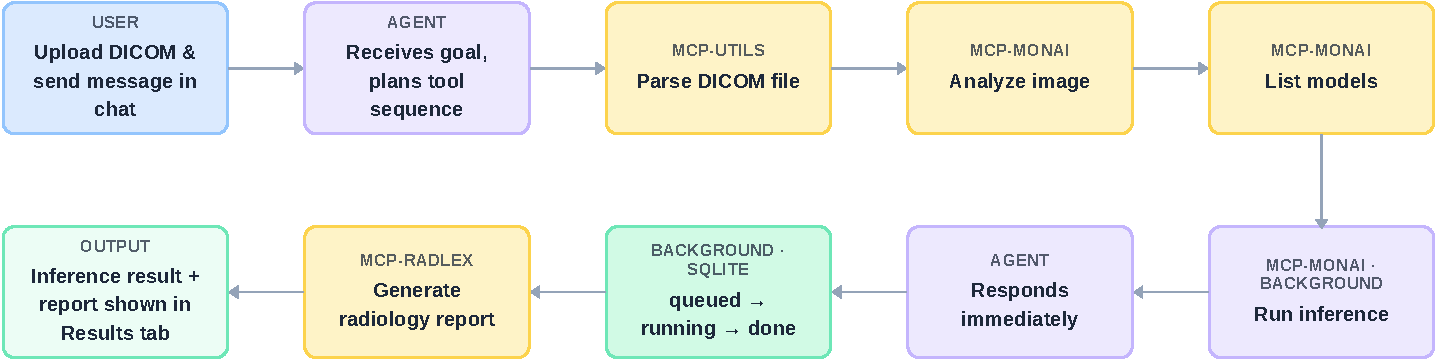
\includegraphics[width=\textwidth]{images/AnalysisWorkflow.pdf}
  \caption{Use Case 1 - Interactive DICOM analysis and segmentation workflow.}
  \label{fig:analysis-workflow}
\end{figure}

\subsection{Use Case 2  -  Interactive WSI Tumor Detection}
A pathologist needs to localize a suspicious region on an histological image, quantify cells within it, and produce a structured pathology report before manually navigating the viewer. Success requires a completed segmentation run with a structured report produced without manual intervention. The user provides a slide UID and prompts: \textit{``Find the tumor in this lung thumbnail (UID: 2.25.3382\ldots869). Identify and localize any suspicious regions consistent with tumor presence. Within the detected tumor area, estimate the number of cells. Then generate a structured report summarizing the findings, including tumor location, size, cell count estimate, and any relevant observations or limitations.''} The agent calls \texttt{ipath.fetch\_thumbnail}, visually inspects it and commits to a bounding box in thumbnail coordinates, then \texttt{ipath.get\_slide\_dimensions} and \texttt{ipath.scale\_roi\_to\_slide} to map it to full resolution, extracts the region with \texttt{ipath.fetch\_roi} (capped at 2700~px per side), then runs \texttt{cellpose.segment\_cells\_2d}. The structured report is written from the \textbf{clinical-reports} pathology template via \texttt{utils.write\_file}.

\subsection{Use Case 3  -  Autonomous Pathology ROI Monitoring}
A pathology instrument or PACS exports ROI images to a directory with no human to initiate analysis. The goal is to detect each new file, run cell segmentation, and route the result by a configurable cell-count threshold, with no user interaction; files may also be dropped manually through the Workspaces tab in the applicationUI. Success requires a completed segmentation and correct routing. The workflow (Figure~\ref{fig:workspace-workflow}) is driven by a configured prompt instructing the agent, for each arriving file, to verify if it is a pathology ROI image, run Cellpose and count cells if so, copy the mask to the output folder when the count exceeds 2000, and otherwise move invalid files to an uncertain folder. On detection the watcher stages the file and triggers the agent after the debounce window; the agent calls \texttt{get\_file\_metadata} and classifies whether the file is a ROI image. Reliable ROI validation would require a dedicated detection model adding an inference step before analysis. To avoid this, the prompt instructs a best-effort classification from metadata and dimensions, routing uncertain cases to a review folder - trading false-negative robustness for efficiency, an acknowledged constraint. If valid, \texttt{segment\_cells\_2d} is queued (cpsam); on completion the result is shown in the Workspaces console, the mask copied to output if the count exceeds 2000 (otherwise a JSON log entry written), and results persisted to the Results tab.

\begin{figure}[H]
  \centering
  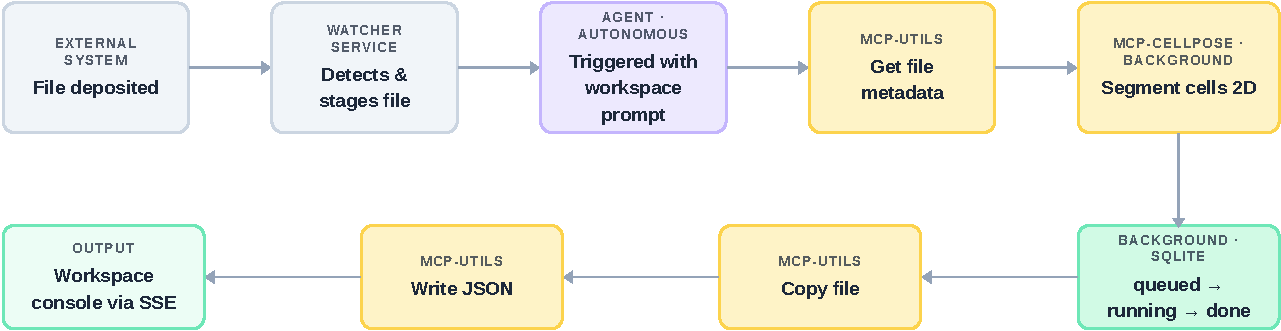
\includegraphics[width=\textwidth]{images/WorkspaceMonitoringWorkflow.pdf}
  \caption{Use Case 3 - Autonomous pathology ROI monitoring workflow.}
  \label{fig:workspace-workflow}
\end{figure}

The dataset for Use Case 1 is the \textbf{Pancreas-CT} collection from TCIA~\cite{tcia}, subject \texttt{PANCREAS\_0001}: 240 DICOM files (121~MB), an abdominal CT volume used without modification. Three MONAI models were evaluated on both hardware configurations (Table~\ref{tab:inference-results}).

\begin{table}[H]
  \caption{MONAI segmentation inference times across hardware configurations for PANCREAS\_0001. 
 M1=\texttt{spleen\_ct\_segmentation}; M2=\texttt{wholeBody\_ct\_segmentation}; M3=\texttt{pancreas\_ct\_dints\_segmentation}.}
  \label{tab:inference-results}
  \centering
  \small
  \resizebox{\linewidth}{!}{%
  \begin{tabular}{llrrrcccc}
    \toprule
    Model & Structure & Voxels & Volume & Scan & Time & Time & Time \\
     &  &  &  (cm$^3$) & \% & (GPU) & (CPU, local) & (CPU, server) \\
    \midrule
    \texttt{M1}          & Spleen         & 57{,}284 & 257.78 & 0.55\% & 9~s   & 27~s    & 25~s \\
    \midrule
    \multirow{3}{*}{\texttt{M2}} & Spleen        & 43{,}402 & 195.31 & 0.42\% & \multirow{3}{*}{18~s} & \multirow{3}{*}{3~m 56~s} & \multirow{3}{*}{3~m 53~s} \\
                                               & Kidney (right) & 30{,}118 & 135.53 & 0.29\% & & & \\
                                               & Kidney (left)  & 17{,}865 &  80.39 & 0.17\% & & & \\
    \midrule
    \texttt{M3} & Pancreas       & 10{,}962 &  49.33 & 0.11\% & 27~s  & 15~m 47~s & 14~m 22~s \\
    \bottomrule
  \end{tabular}}
\end{table}

\section{Results}
\label{sec:results}

\subsection{Phase 1  -  Model Experimentation}
Five models were evaluated: three API-based (Gemini 2.0 Flash, 2.5 Flash, 3.0)~\cite{gemini2025} and two local (deepseek-r1:7b~\cite{deepseekr1}, llama3.1:8b~\cite{llama31}). The loop was capped at 10 iterations; a model that does not signal \texttt{goal\_achieved} within that budget fails regardless of correct individual tool selections.

Both local models were tested at 30W and 60W. At 30W tool selection was generally correct on the first attempt, but neither model reliably reached \texttt{goal\_achieved} within the limit: they selected correct tools but failed to chain them into a complete workflow. At 60W outcomes were mixed. Across profiles, local models rarely recovered from a failed call by trying an alternative, confirming the need for the repetition guard. Each local call took $\approx$20~s of inference, making a 10-iteration task up to three minutes of model time alone - a constraint of model scale, not configuration. A key finding is that two architectural choices significantly influenced reliability regardless of profile: the quality of tool descriptions (without clear descriptions, models defaulted to plausible but incorrect selections) and the availability of stateful execution history (without it, models repeated failing calls). Both apply equally to the API backend.

Gemini 2.0 and 2.5 Flash resolved all reliability issues, completing multi-step workflows within the budget, correctly sequencing calls, and recovering from failures by selecting alternatives. API inference per iteration was near-instant versus $\approx$20~s locally, reducing completion time by an order of magnitude; MCP tool execution time is identical across backends since tools run locally. The primary API limitations are external - availability outside the system's control, and transmission of all submitted data to a third party. Token consumption is a further consideration: because the agent passes its execution history back each iteration, usage grows per call, and early mistakes (passing image bytes directly, or returning all file paths from \texttt{parse\_dicom\_directory}) inflated single calls by tens of thousands of tokens. Several measures manage this growth: Gemini's stateful session mode, MCP sampling for report narratives (a lateral call outside the agent's context), removal of \texttt{get\_template\_schema}, and skills' progressive disclosure.

The architecture is backend-agnostic and functions with both; the gap is task-completion reliability at current local scales. Local models at 7--8B select appropriate tools but cannot reliably complete multi-step workflows within a bounded budget, whereas larger API-hosted models resolve this reliably (Table~\ref{tab:model-comparison}).

\begin{table}[H]
  \caption{Language Model Comparison for Agentic Tool-Calling}
  \label{tab:model-comparison}
  \centering
  \begin{tabular}{llll}
    \toprule
    Model & Type & Time/call & Task completion \\
    \midrule
    deepseek-r1:7b (30W) & Local & $\approx$20s & Failed within 10 iter. \\
    llama3.1:8b (30W)    & Local & $\approx$20s & Failed within 10 iter. \\
    Both models (60W)$^{a}$ & Local & $\approx$20s & Partial \\
    Gemini 2.0 Flash     & API   & $<$1s        & Consistent \\
    Gemini 2.5 Flash     & API   & $<$1s        & Consistent \\
    \bottomrule
  \end{tabular}
  \par\smallskip
  \raggedright\footnotesize
  $^{a}$~Both deepseek-r1:7b and llama3.1:8b produced equivalent mixed results at 60W and are combined into a single row.
\end{table}

\subsection{Phase 2  -  Autonomous Agent Execution}
This phase tests whether loading a skill changes tool selection and whether the prescribed sequence is followed autonomously. Using the \textbf{dicom-analysis} skill the agent receives an explicit sequence (parse header, \texttt{analyze\_image}, filtered \texttt{list\_models}, download if needed, then queue inference), each step a guard condition for the next. With the skill active, the agent followed the sequence without deviation across all 10 runs (10/10); on one run where \texttt{analyze\_image} returned an ambiguous modality, it called \texttt{list\_models} with both candidates before selecting. Without the skill it also completed 10/10, but occasionally skipped the analysis step and inferred parameters from the filename - correct in straightforward cases but fragile for non-descriptive names or atypical metadata. One deployment trace shows the agent autonomously handling an unrecognised file: it attempted \texttt{monai.analyze\_image} (header error), created an \texttt{uncertain/} directory, moved the file, and called \texttt{goal\_achieved} in six iterations, confirming graceful failure handling. Skills are thus not required to complete tasks but are what make autonomous execution \emph{reliable}, constraining the agent to the correct sequence and preventing plausible but clinically incorrect shortcuts.

The same DICOM task was executed in assisted and autonomous mode with identical goal, files, and skill. The tool-call sequences were identical - same tools, same order, same arguments, same iteration count - and no call was rejected or modified during the assisted run. Had assisted mode been a correction mechanism, the sequences would have diverged on override; they did not, indicating the agent's autonomous decisions were already correct and confirmation added visibility without changing the outcome. Assisted mode is therefore a transparency mechanism, not a safety net, which supports autonomous mode for event-driven workflows where no user is present.

\subsection{Phase 3  -  Use Case Comparison}
Use Cases 1 and 2 were each executed under two conditions to isolate the effect of workflow guidance: a \emph{skilled} condition (agent loads and follows the skill) and an \emph{unskilled} condition (agent selects tools from general reasoning over tool descriptions). %Use Case 1 used the TCIA series; Use Case 2 used the iPath slide UID. 
Results are summarised in Table~\ref{tab:uc1-results}.

\begin{table}[H]
  \caption{Use Cases 1 and 2: Execution Metrics and Outcomes}
  \label{tab:uc1-results}
  \centering
  \resizebox{\linewidth}{!}{%
  \begin{tabular}{lrrrrccp{4cm}c}
    \toprule
    Use Case & Iter. & 1st-iter. & Total & Time & Success  & Completed & Final result & Incorrect  \\
     &  & tok. & tok. & (s) & rate &  &  &  calls \\
    \midrule
    1               & 6 & 8{,}204  & 80{,}961  & 58.3  & 10/10 & Yes     & Spleen 192.51~cm$^{3}$, radiology report       & None \\
    1 w/ skill      & 8 & 8{,}251  & 90{,}973  & 95.1  & 10/10 & Yes     & Spleen 192.51~cm$^{3}$, radiology report       & None \\
    2               & 8 & 8{,}158  & 95{,}942  & 117.9 & 0/10  & Partial & Cell segmentation done; report in wrong domain & $^{a}$ \\
    2 w/ skill      & 9 & 8{,}237  & 135{,}842 & 129.6 & 10/10 & Yes     & 428 cells detected, pathology report           & None \\
    \bottomrule
  \end{tabular}}
  \par\smallskip
  \raggedright\footnotesize
  $^{a}$~\texttt{radlex.generate\_radiology\_report} applied to pathology specimen.
\end{table}

In Use Case 1, both conditions completed successfully: the agent parsed the DICOM directory, identified an abdominal CT, selected a compatible model, and queued inference, with spleen segmentation yielding 192.51~cm³ and a valid RadLex report in each run. The skilled condition required two extra iterations for the prescribed steps, raising total tokens from 80{,}961 to 90{,}973 and time from 58.3~s to 95.1~s with no difference in clinical output.

Use Case 2 produced a stark contrast. Both conditions executed the full segmentation sequence, but the unskilled agent called a radiology report tool on a pathology image, yielding a template inapplicable to a tissue specimen (Figure~\ref{fig:task2-noskill-report}) - a partial outcome: segmentation completed, but the report was produced in the wrong domain. With the \textbf{wsi-tumor-detection} skill active, the agent followed the sequence without deviation, detected 428 cells in the 2{,}700$\times$2{,}700~px ROI, and generated a pathology report from the \textbf{clinical-reports} template (Figure~\ref{fig:task2-skill-report}), consuming 135{,}842 tokens against 95{,}942 for two skill files. Use Case 2 thus confirmed the skill was not merely beneficial but \emph{necessary}: the skilled condition succeeded 10/10 while the unskilled condition failed every run (0/10), producing domain-incorrect reports each time.

\begin{figure}[H]
  \centering
  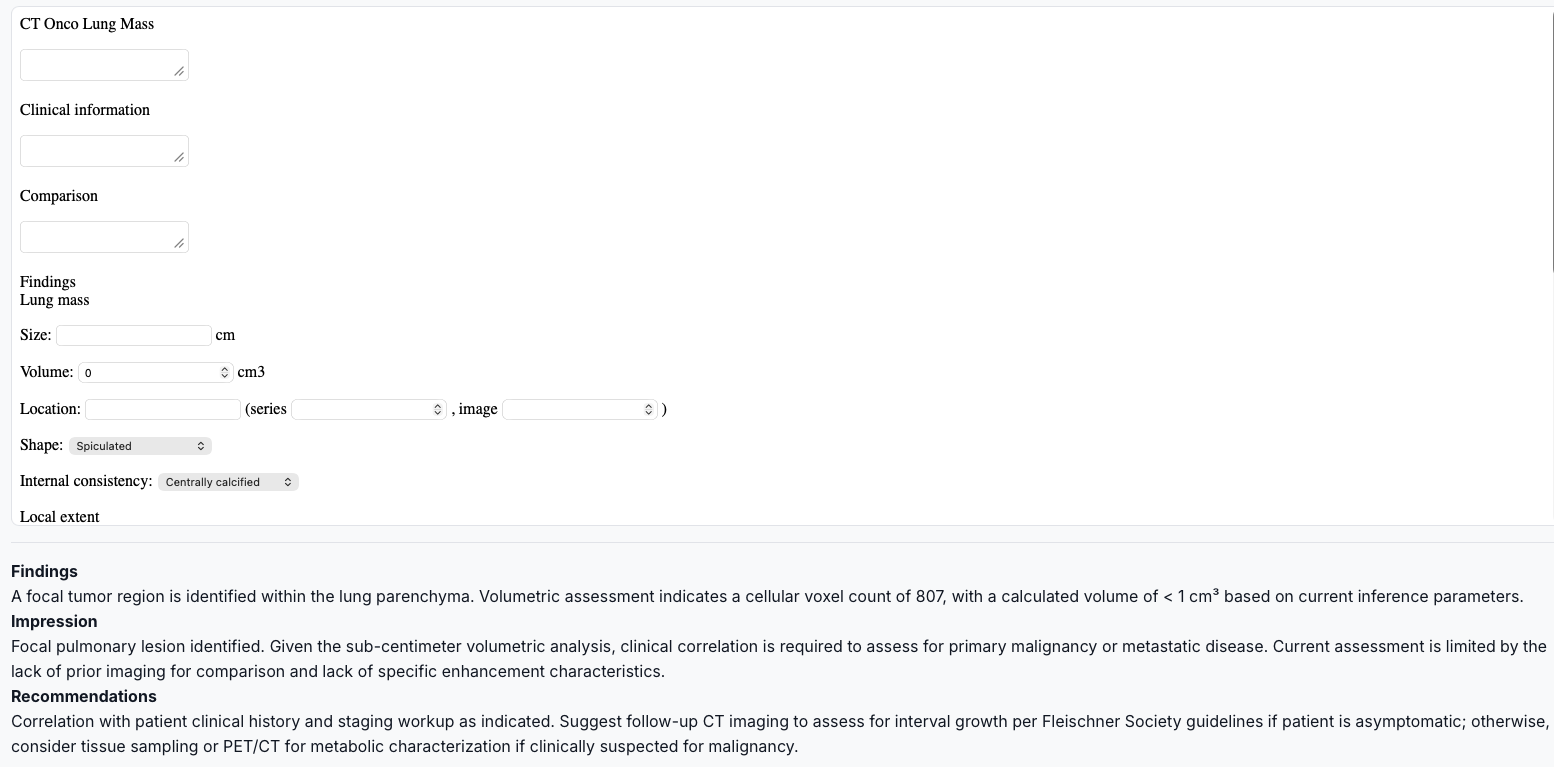
\includegraphics[width=\linewidth]{images/uc2-noskill-report.png}
  \caption{Use Case 2: the agent applied a radiology report template to a pathology specimen, producing fields inapplicable to tissue analysis.}
  \label{fig:task2-noskill-report}
\end{figure}

\begin{figure}[H]
  \centering
  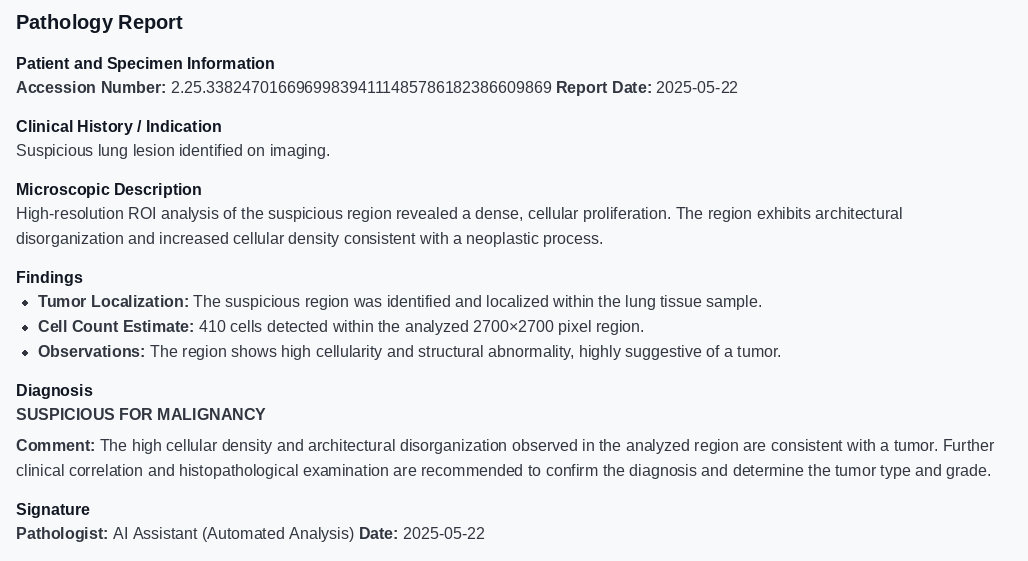
\includegraphics[width=\linewidth]{images/uc2-skill-report.png}
  \caption{Use Case 2 with skill: the \textbf{wsi-tumor-detection} skill directed the agent to use the pathology template from \textbf{clinical-reports}, producing a report with specimen information, microscopic description, and diagnosis fields appropriate to a tissue specimen.}
  \label{fig:task2-skill-report}
\end{figure}

For Use Case 3, two workspaces validated the trigger pipeline and instruction following without cross-routing. The \textbf{CELLPOSE} workspace was given a no-op prompt (\textit{``Do nothing, just a placeholder for images.''}); deposited files produced no action, confirming no bias toward running tools when the prompt does not call for it. The \textbf{ROI} workspace was configured verbatim: \textit{``To this folder there will arrive ROI images, I want you to count the number of cells for each image that arrives and I want that if the number of cells counted is above 100 to send the image to the folder in /app/workspaces/CELLPOSE.''} When \texttt{ROI\_TEST\_IMAGE.jpeg} (2{,}352$\times$2{,}673~px, H\&E ROI) was deposited (Figure~\ref{fig:workspace-use-case}), the watcher detected it within seconds, triggered the agent after the debounce window, and the agent autonomously called \texttt{cellpose.segment\_cells\_2d}, reported 1{,}706 cells, and - exceeding the threshold - moved the image to CELLPOSE as instructed. The full sequence took $\approx$30~s on a local GPU (RTX 3050), confirming end-to-end operation of the watcher, debounce trigger, tool selection, and cross-workspace routing via a plain-language rule.

\begin{figure}[H]
  \centering
  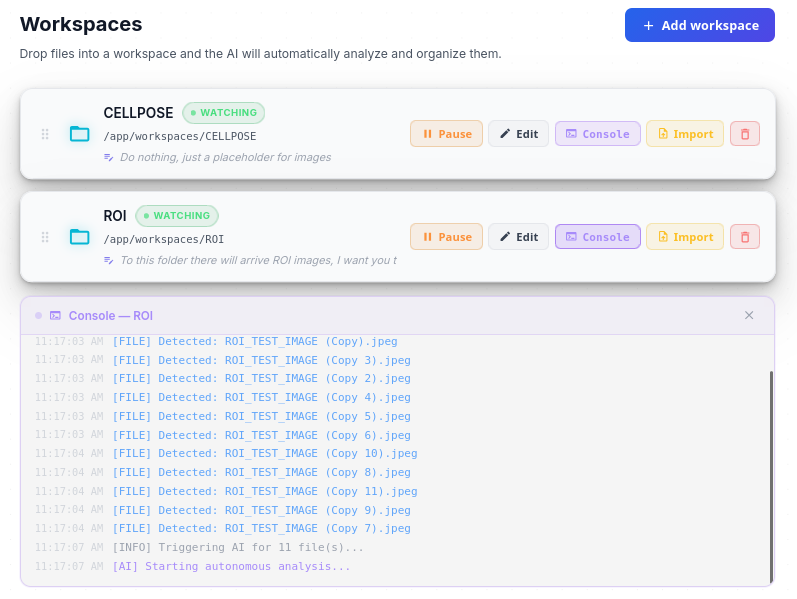
\includegraphics[width=\linewidth]{images/workspace_use_case.png}
  \caption{Workspace console showing autonomous detection and routing: ROI\_TEST\_IMAGE.jpeg detected, 1{,}706 cells counted, image moved to CELLPOSE workspace.}
  \label{fig:workspace-use-case}
\end{figure}

\subsection{Inference Hardware Requirements}
Inference performance is tightly coupled to hardware, with direct clinical implications (Table~\ref{tab:inference-results}). Cellpose v4 (cpsam) is a SAM-based architecture designed for GPU: on CPU, a 64$\times$64 test image took 95~s, and a real ROI (2{,}352$\times$2{,}673~px) took 12~m~37~s on a local Ryzen 5 8645HS and ran $\approx$3~h on the server before hanging. MONAI times are nearly identical across machines because the server pins to a single thread (\texttt{OMP\_NUM\_THREADS=1}, \texttt{MKL\_NUM\_THREADS=1}), whereas Cellpose scales with cores and the 4-core VM introduces order-of-magnitude overhead. On GPU the same ROI completed in 30~s (RTX 3050, local) and 28~s (RTX 3060, server), eliminating the VM bottleneck. GPU execution is thus a practical prerequisite for the pathology use case~\cite{cellpose}. The MONAI pipeline is similarly GPU-dependent: on the RTX 3050 (6~GB), some models exceeded VRAM and the subprocess terminated without output, diagnosed only after adding stderr capture to surface the PyTorch out-of-memory exception. The system therefore ships with a GPU-enabled Docker configuration as the recommended target, with CPU fallback for development only.

A practical advantage independent of accuracy is convenience: regardless of hardware, long-running operations are queued automatically and results persisted, so the clinician can return to completed outputs without having been present - directly enabling overnight or unattended processing. Meaningful evaluation of this property at scale requires a broader set of datasets and input types, an important direction for further work.

\section{Discussion}

\subsection{MCP as a Practical Integration Layer}
Section~\ref{sec:introduction} identifies fragmentation as a structural problem: AI tools exist but no standard layer connects them. The developed framework and our results support MCP as a candidate solution. Six servers covering distinct capabilities were integrated without any agent-side connector code, and adding a server required no agent changes. This composability held under real conditions: all three use cases required dynamic sequencing across multiple servers, and the agent did so correctly without hardcoded knowledge of their implementations. The broader implication is that MCP could reduce the integration overhead that slows clinical AI adoption. The integration contract is the protocol, so a conforming server is immediately accessible to any conforming agent, shifting the bottleneck from integration engineering to tool capability, a more tractable problem. Singh et al.\ argue this conceptually~\cite{mcp-aditi}; our use cases provide evidence in practice.

One finding qualifies this: MCP decouples the agent from a server's implementation, but not from the quality of each tool's natural-language description. Vague descriptions caused incorrect selections even when the correct tool was available - consistently with local models, less so with API models - so the integration problem is partly displaced from adapter code to description authorship. Skills partially compensate; when active, the agent follows an explicit protocol naming specific tools, reducing dependence on description quality~\cite{agentskillslargelanguage}. MCP and skills are therefore complementary, and neither alone is sufficient for complex workflows. An open question is scaling beyond six servers: all descriptions are loaded into context at startup, and as the catalogue grows, selection from a larger set is expected to degrade. Skills as workflow guides partially mitigate this but do not reduce the tool list itself; a multi-agent architecture where specialists expose only domain-relevant tools is a natural extension left to future work~\cite{klang2026orchestrated}.

\subsection{Skills as Workflows: When Guidance Changes Behaviour}
Use Cases 1 and 2 clarify when a workflow skill changes behaviour. In Use Case 1 the skill made no difference: with no ambiguous decision fork, the agent reached the correct sequence through general reasoning, and the skill only enforces protocol adherence (valuable for reproducibility). Use Case 2 produced a clinically incorrect decision without the skill, illustrating the mechanism by which a workflow skill corrects agent behaviour: a \emph{domain selection failure} in which the agent called \texttt{radlex.generate\_radiology\_report} on a pathology specimen. The reason follows from how the system exposes tools and skills differently at startup: \texttt{radlex.generate\_radiology\_report} is a directly callable MCP tool whose full name, schema, and description are visible from the moment the session begins, while the \texttt{clinical-reports} skill is known only by its short description until explicitly loaded; its internal templates are invisible until the agent decides to open it. Without a workflow directing that loading step, the agent selected the most visible tool matching the goal of generating a report, with no mechanism to detect the domain mismatch from descriptions alone. The skill resolved this by prescribing the correct template and ruling out the radiology tool, a routing decision the agent could not reach on its own. Skills as workflows are thus most valuable at decision forks where a plausible but incorrect option exists; where none exists, their value is limited to reproducibility.

\subsection{Clinical Accuracy and Validation Scope}
This evaluation measures task completion - whether the agent orchestrated the required tools, followed the workflow, and produced an output - not clinical correctness, and conflating the two would overstate the contribution. Segmentation accuracy for the models used is established in their own benchmarks. What is not evaluated is whether the agentic layer introduces errors absent from direct invocation: consistent model selection, appropriate inference parameters, and correct mapping of findings to report fields. These orchestration-specific failure modes require dedicated validation, e.g., a comparison against radiologist ground truth, Dice scores across a representative dataset, and testing across institutions and protocols. Until then, the system should be understood as a workflow automation tool that reduces orchestration effort, not a clinically validated decision-support system - a distinction common to any agentic layer over existing models, but one that must be stated explicitly.

\subsection{Privacy vs Reliability in Clinical Deployment}
The results expose a tension with no clean resolution: Cloud API models completed workflows reliably, while local 7--8B models did not, so reliable autonomous operation currently entails transmitting clinical metadata, including DICOM patient identifiers, to a third party, a significant concern under GDPR and HIPAA. The two properties that matter most for adoption, privacy and reliability, pull in opposite directions under current constraints. This reflects the resources available here rather than local-model capability in general: larger open-weight models exist but require GPU resources beyond most deployments. The architecture supports both backends unchanged, so the limitation is specific to the 7--8B models tested. A sufficiently capable local model would satisfy both requirements, and the same architecture would benefit as accessible hardware improves. Several paths could close the gap: fine-tuning a smaller model on clinical tool-calling sequences, on-premise deployment of larger models where the privacy requirement justifies the investment, or a hybrid where a local model handles routing and an API model is invoked only for complex reasoning on de-identified data~\cite{trustworthyai2025, dietrich2025agentic, agiformedicalimaging2025}.

\section{Conclusion}
This work demonstrates that an agentic AI system using MCP as a standardized interoperability layer can autonomously orchestrate multi-step clinical imaging workflows without custom integration code. All three use cases completed end-to-end without manual intervention, six MCP servers were integrated without agent-side connector code, and the skill-based governance mechanism demonstrably changed agent behaviour in the pathology task, preventing domain-incorrect tool selection that occurred without it. Assisted and autonomous modes produced identical tool sequences, indicating the agent's decisions were correct independently of human oversight and supporting unattended operation for event-driven workflows.

The comparison between cloud and local models exposed a tension clinical deployment cannot currently avoid: reliable multi-step tool-calling requires model scale exceeding what most institutions can run locally, yet transmitting clinical data to an API raises GDPR/HIPAA concerns. This reflects the current state of open-weight capability relative to available resources; a hybrid local/API approach on de-identified inputs is a concrete direction for resolving it. Logging and auditing, implemented as a transparency mechanism, proved more valuable than anticipated. The workspace console's step-by-step trace was essential for diagnosing failures and building confidence in unattended operation, and such traceability will become a compliance requirement as agentic systems take on more consequential tasks. Security, such as tool-level access control and audit-trail integrity, was not a focus here but is necessary before production deployment.

Future work includes token-consumption optimization through smarter history pruning and selective skill loading, prompt engineering and fine-tuning smaller models on clinical tool-calling to close the reliability gap, and a dedicated worker process per GPU for multi-tenant scale. Most importantly, the evaluation here measures orchestration correctness, not clinical accuracy. Before any real clinical use, rigorous validation requires Dice comparisons against ground truth, prospective testing across institutions, and clinician review. 

The broader contribution is a demonstration that MCP combined with a skills system for domain-specific governance provides a practical, extensible integration layer for clinical AI. Any tool wrappable in an MCP server becomes immediately accessible to the agent, and as more tools adopt MCP the integration overhead that limits adoption shifts from adapter engineering to tool capability itself. %A working deployment of MedGov-AI is publicly accessible at \url{https://medgovai.bmd-software.com/}.

\section{Acknowledgements}
This work has received support from the “Health from Portugal - Agenda Mobilizadora para a Inovação Empresarial” project, funded by the Portuguese PRR under grant agreement No C644937233-00000047.

\bibliographystyle{elsarticle-num}
\bibliography{references}

\end{document}
